% !TEX root = ../main.tex

\subsubsection{Sensitivity to Initial Perturbations}

We next compare the sensitivity of the three linearized models to increasing initial-condition perturbations. In this experiment, we use the baseline normalized weighting matrices and compare: (i) the hover linearization, (ii) the nominal descent linearization without attitude coupling, and (iii) the nominal descent linearization with prescribed attitude coupling.

Let \(\delta x_{\mathrm{base}}(0)\) denote the reference initial perturbation. For each perturbation scale \(\gamma>0\), we initialize the linearized system at
\[
    \delta x(0;\gamma)
    =
    \gamma\delta x_{\mathrm{base}}(0).
\]
For each value of \(\gamma\), we solve the finite-horizon LQR problem and record the resulting state response and control perturbation energy. This experiment compares how the three linearized models respond as the initial deviation from the corresponding nominal trajectory increases.

\begin{figure}[htbp]
    \centering
    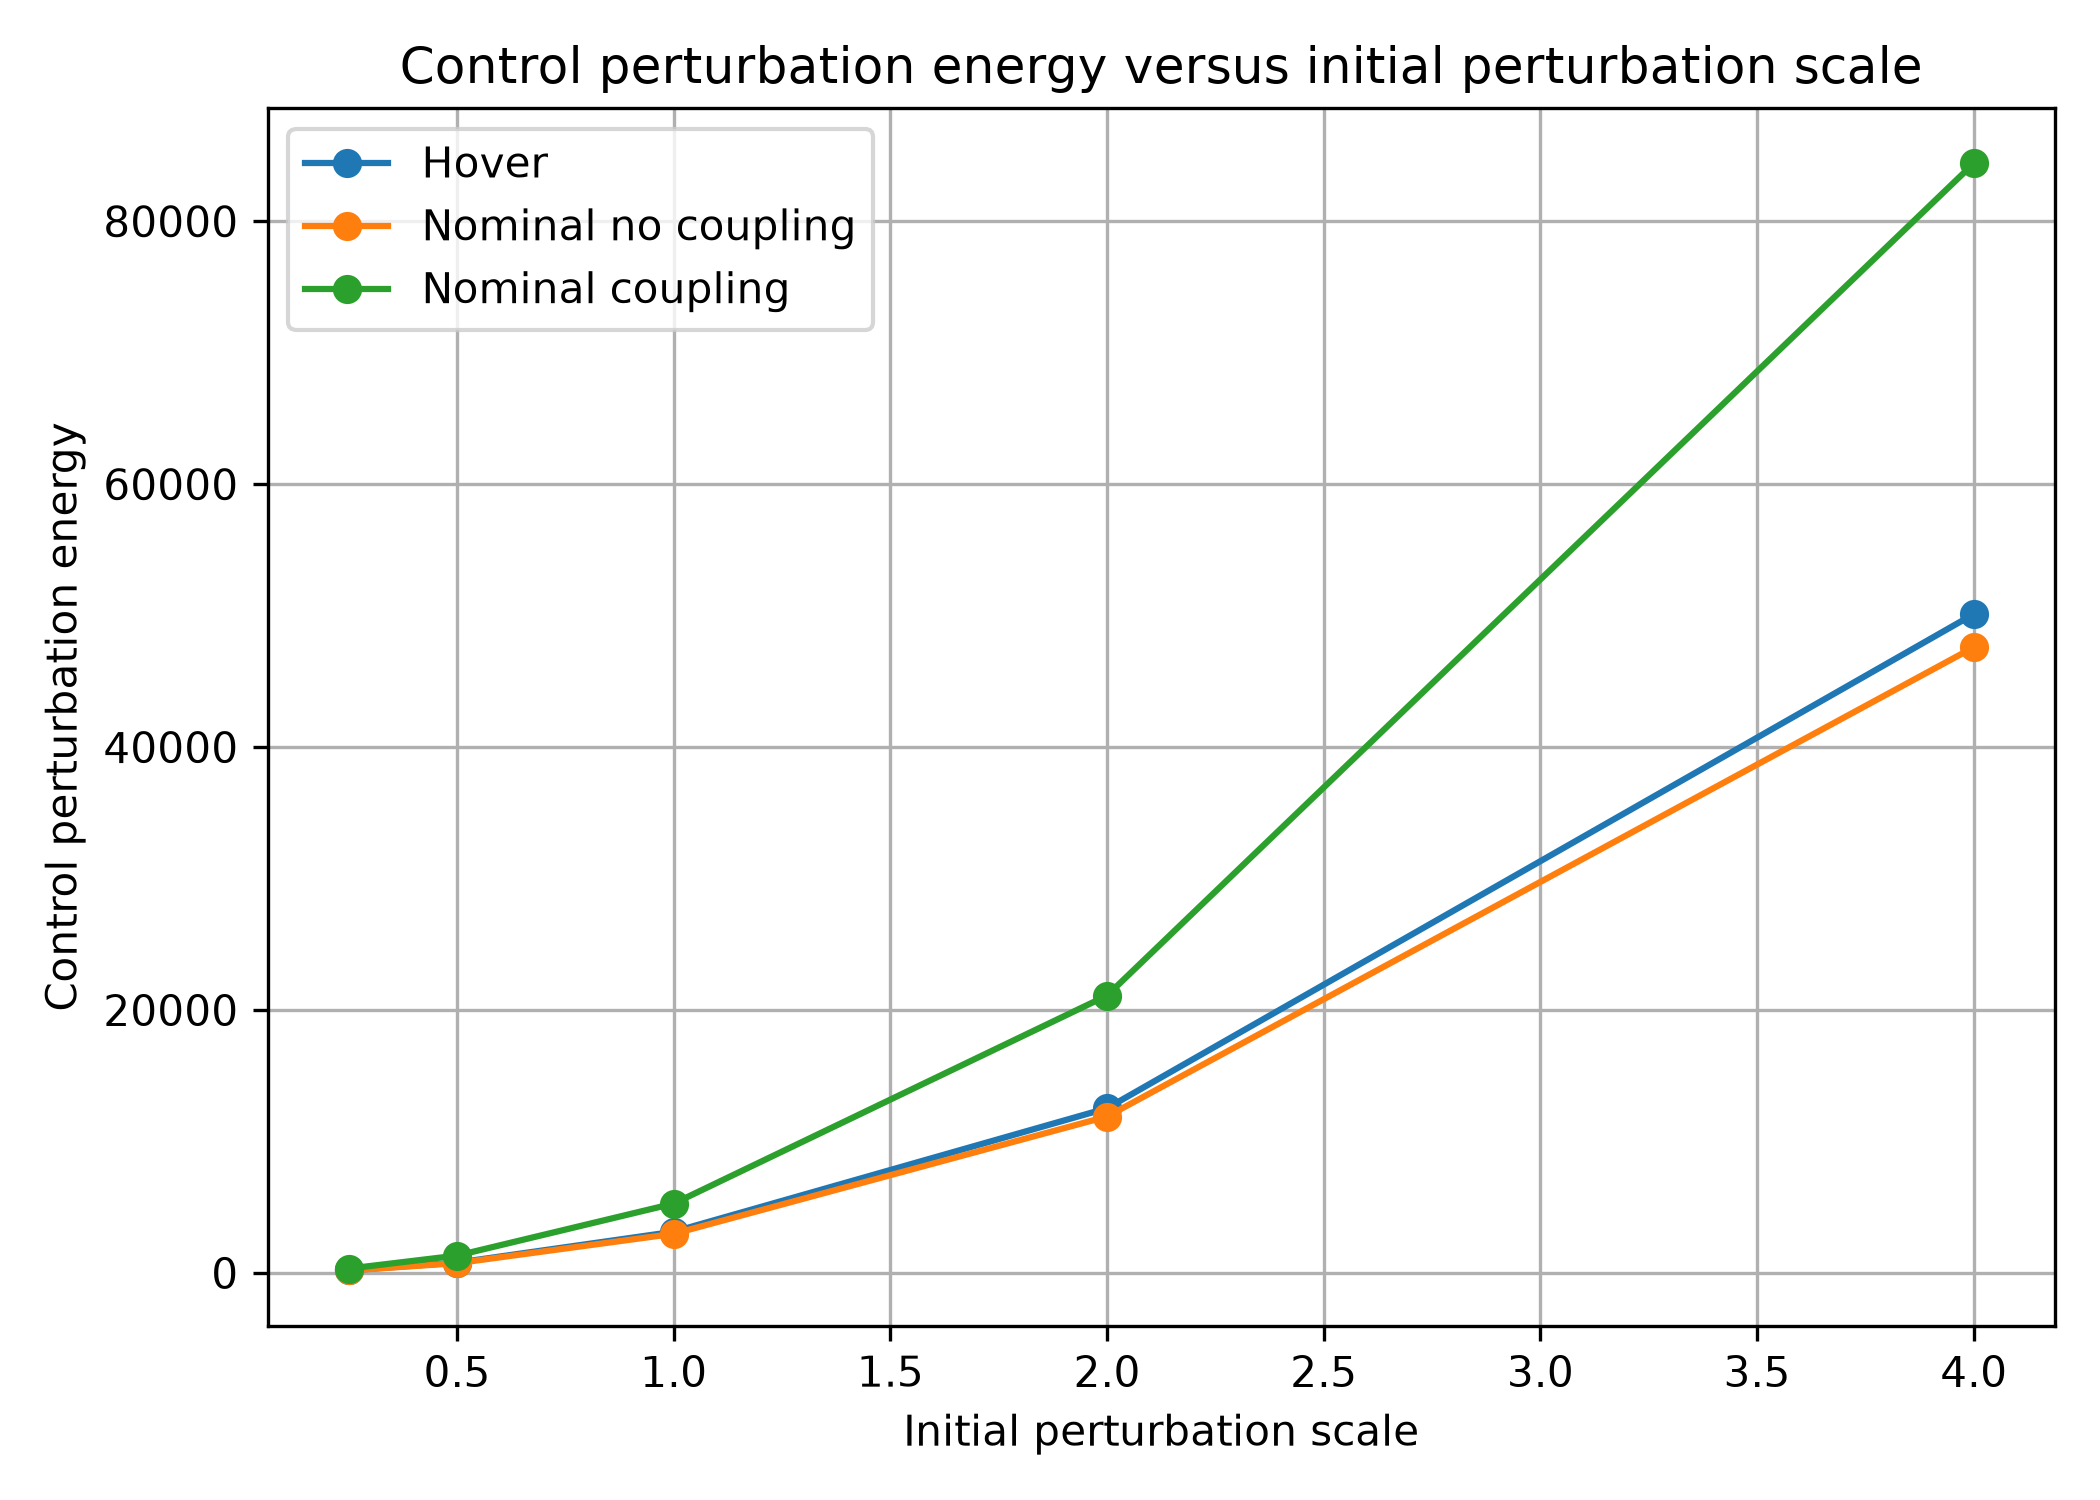
\includegraphics[width=0.90\columnwidth]{sections/PART5C/control_energy_vs_scale.png}
    \caption{State perturbation norm \(\|\delta x(t)\|_2\) for perturbation scale \(\gamma=1\).}
    \label{fig:state-norm-scale1}
\end{figure}

\begin{figure}[htbp]
    \centering
    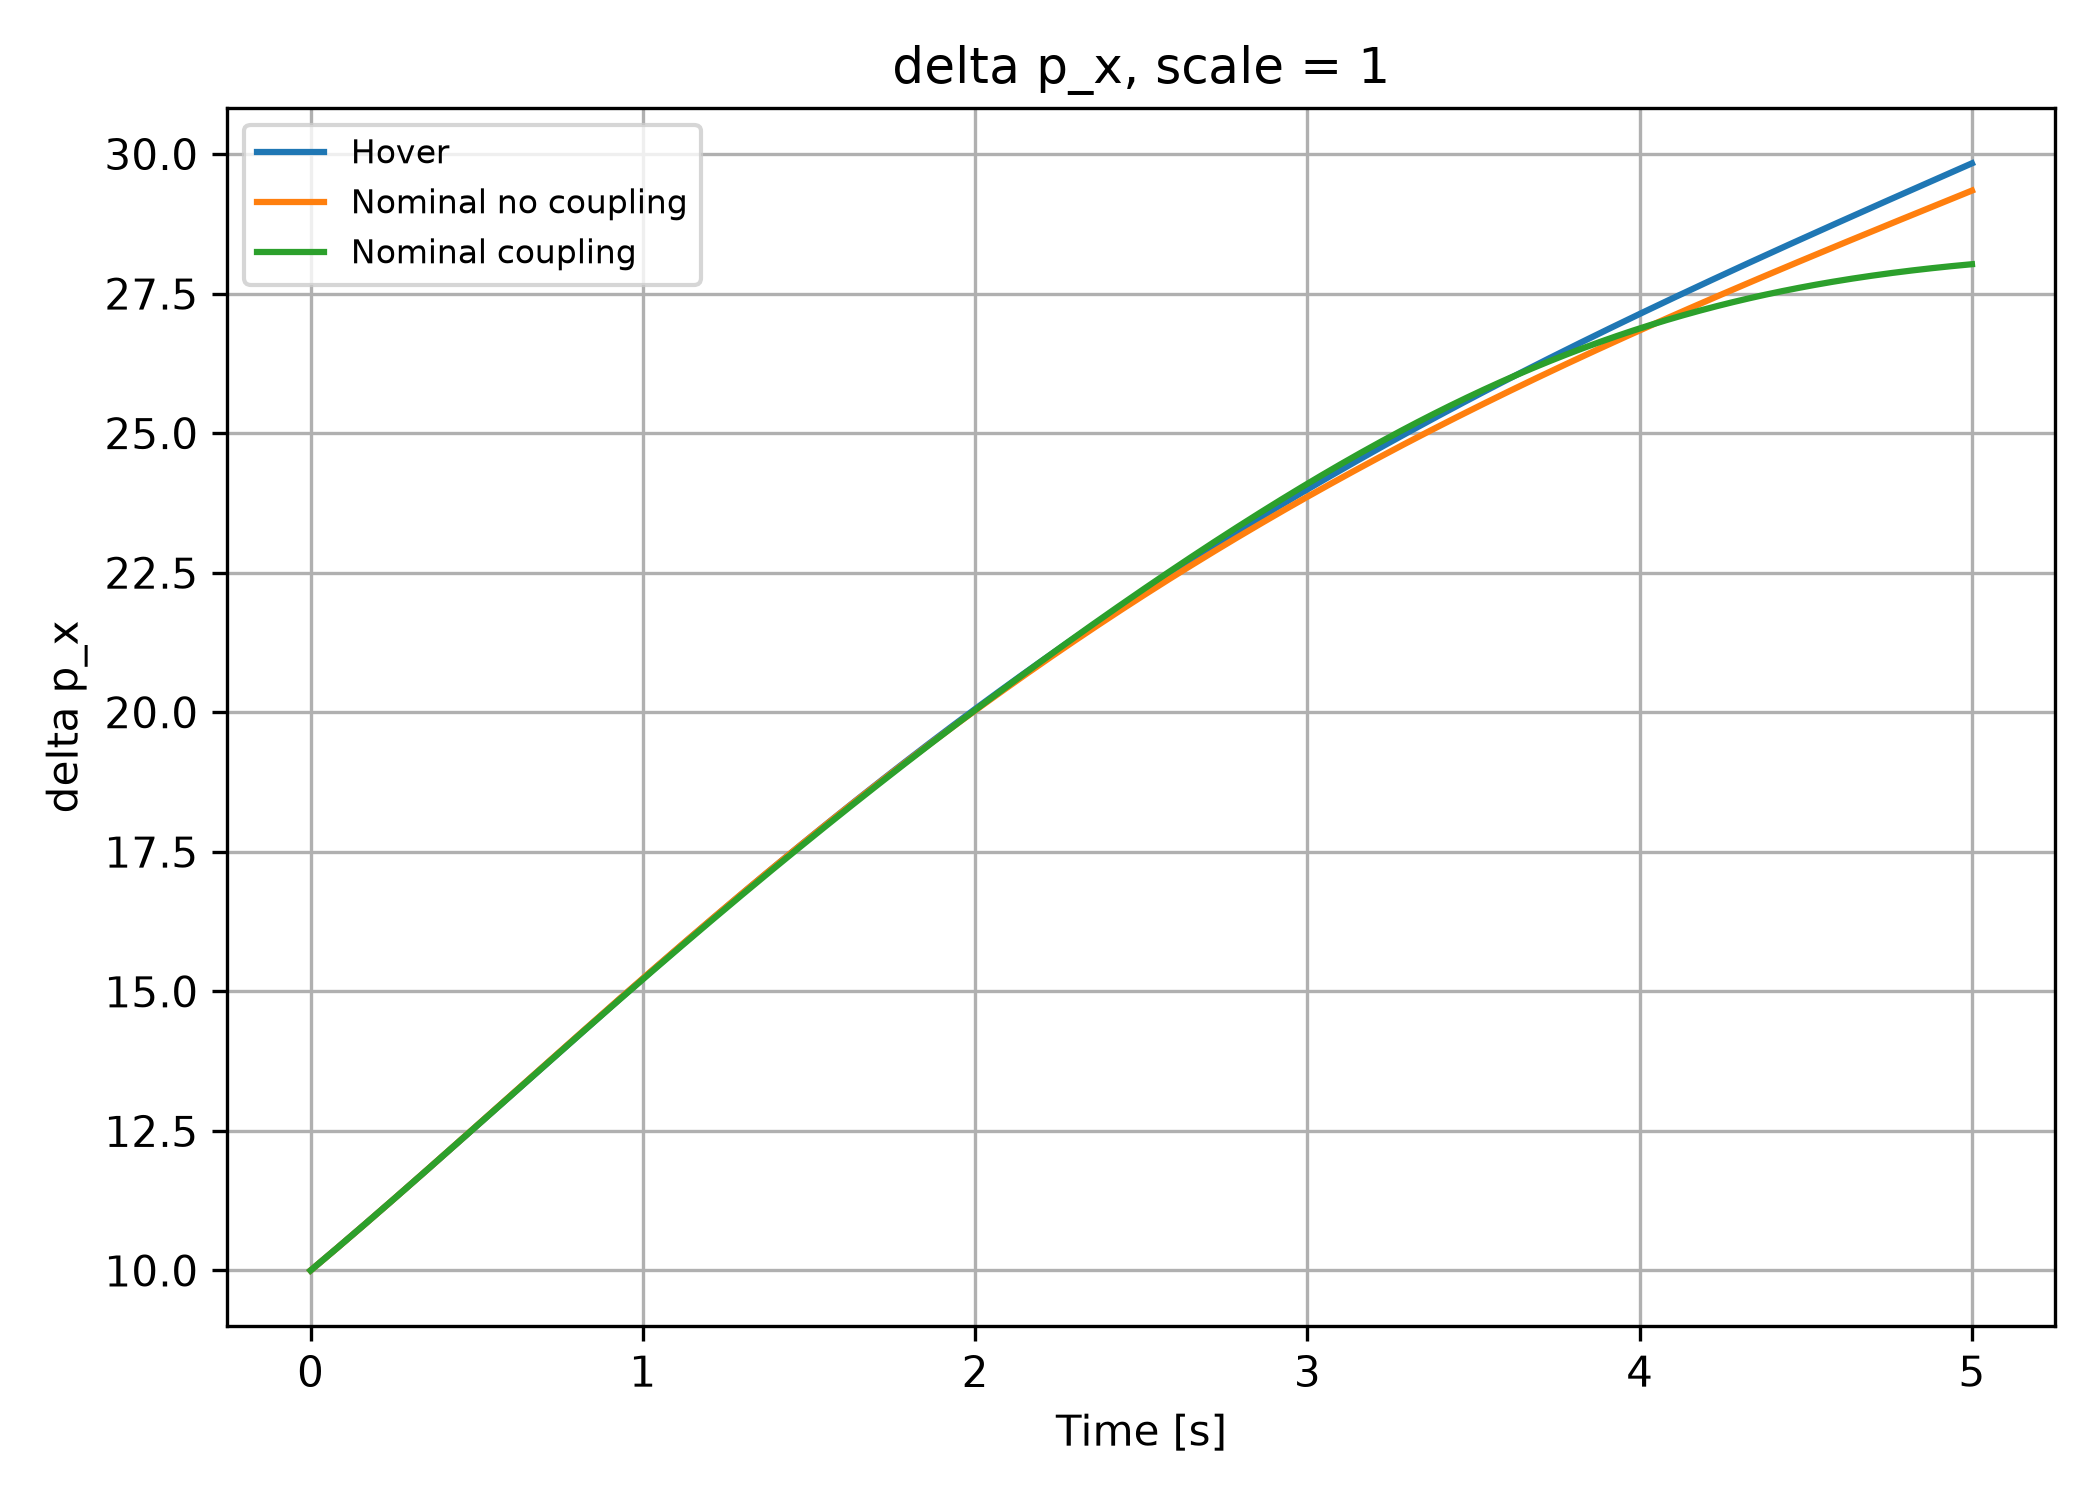
\includegraphics[width=0.90\columnwidth]{sections/PART5C/delta_p_x_time_history_scale_1p0.png}
    \caption{Horizontal position perturbation \(\delta p_x(t)\) for perturbation scale \(\gamma=1\).}
    \label{fig:px-scale1}
\end{figure}

\begin{figure}[htbp]
    \centering
    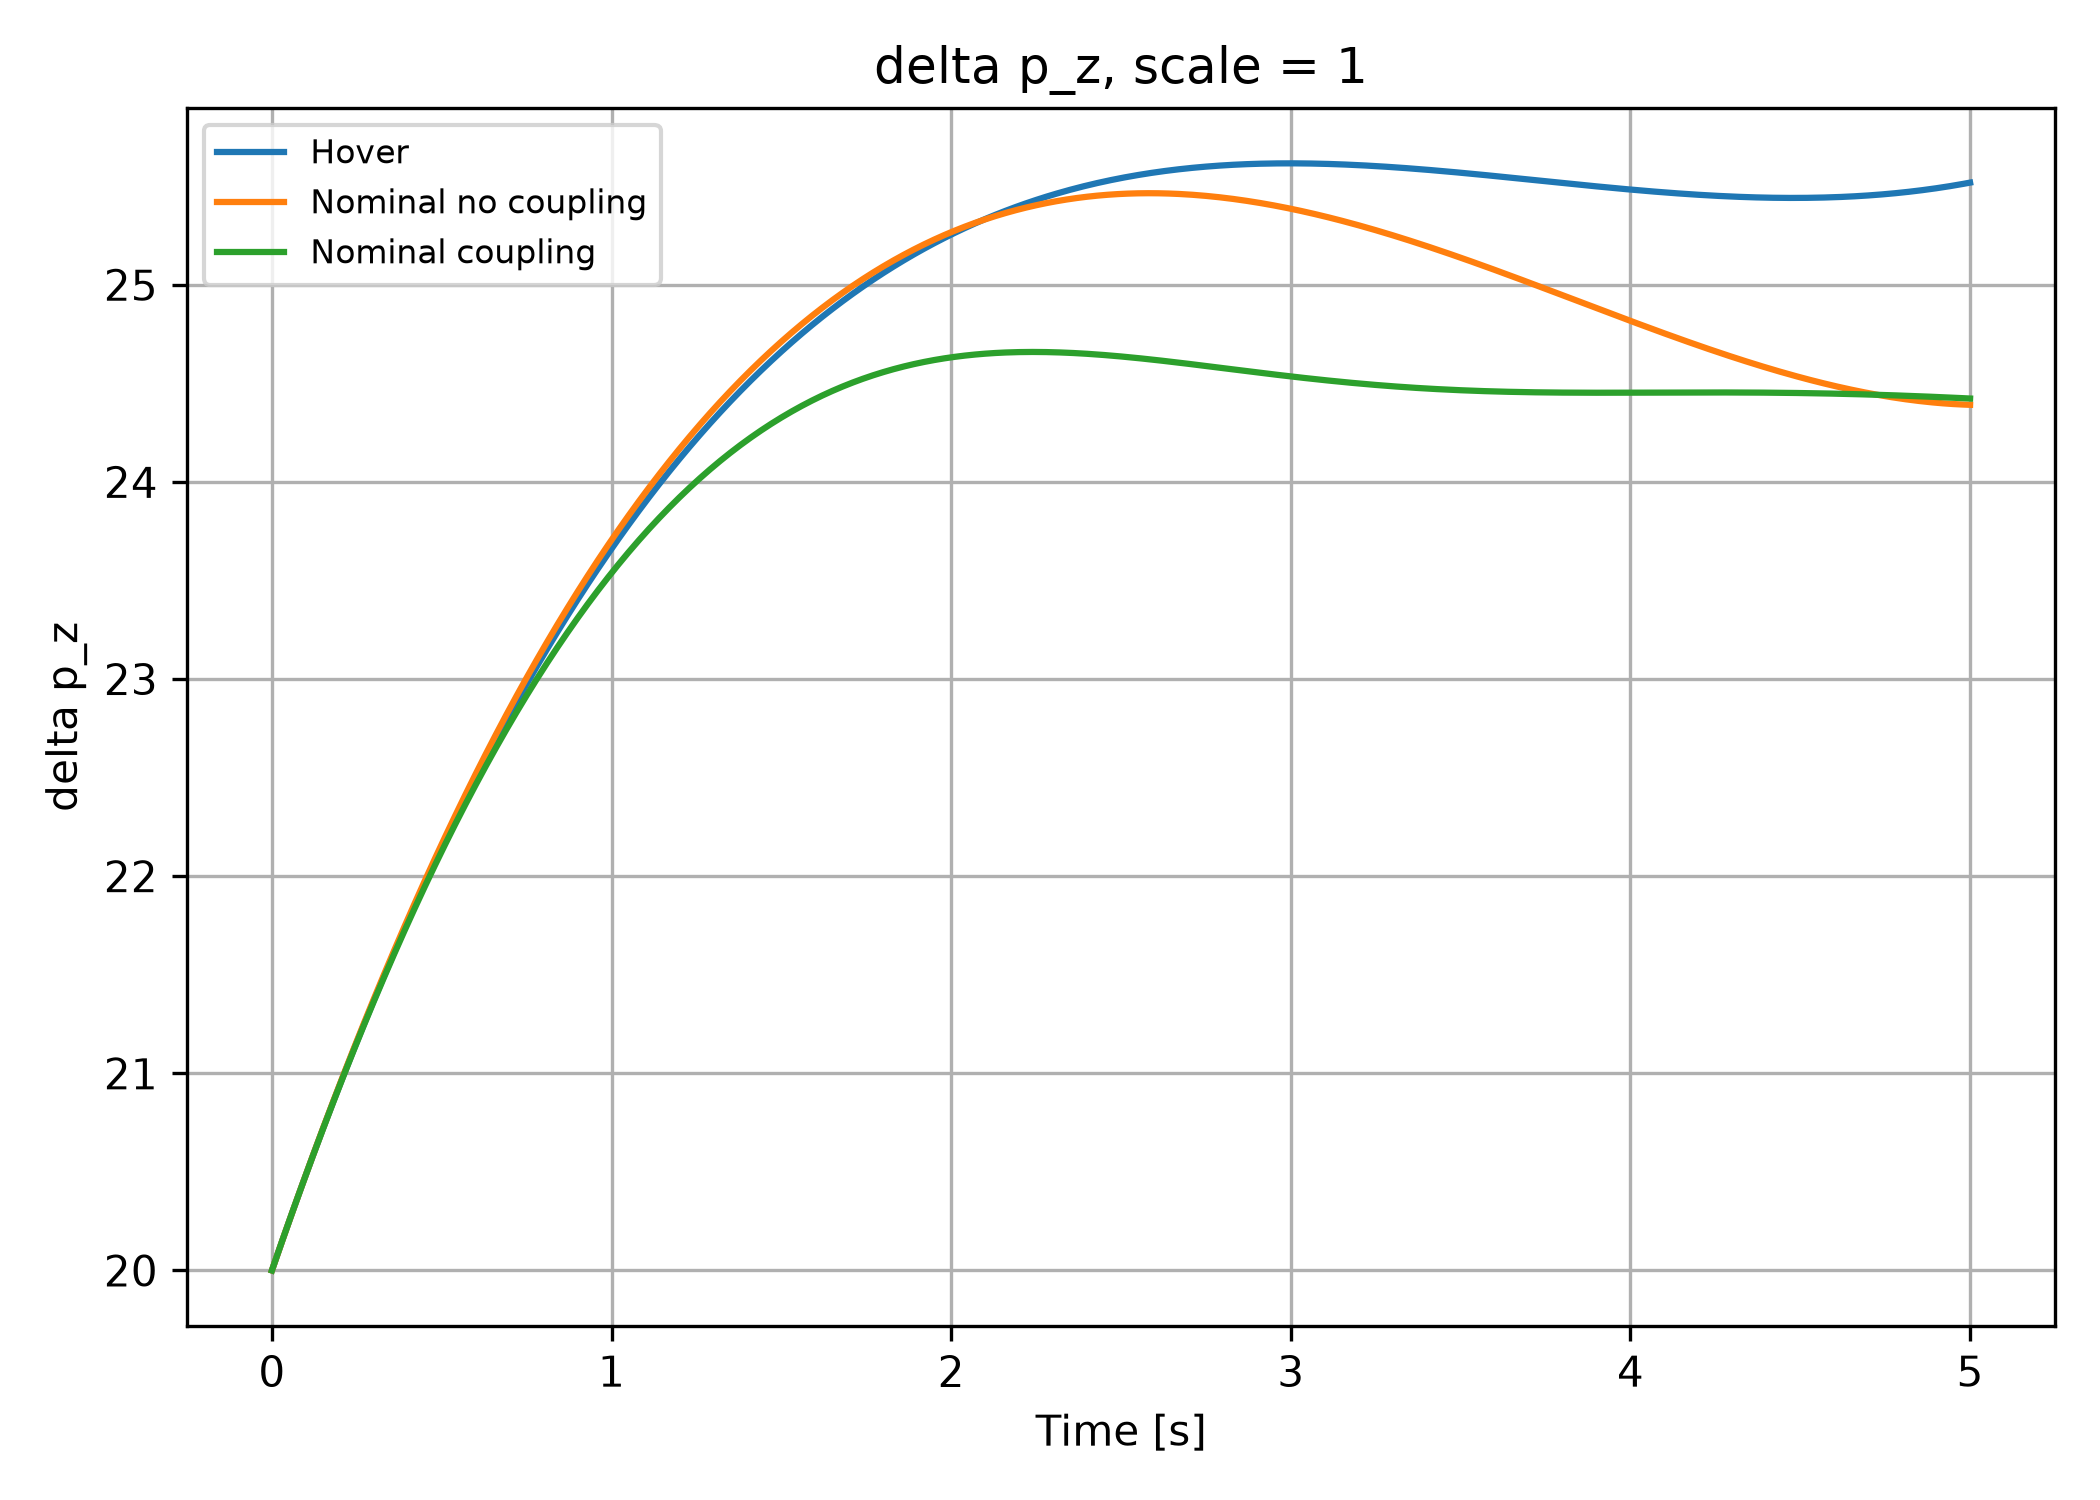
\includegraphics[width=0.90\columnwidth]{sections/PART5C/delta_p_z_time_history_scale_1p0.png}
    \caption{Vertical position perturbation \(\delta p_z(t)\) for perturbation scale \(\gamma=1\).}
    \label{fig:pz-scale1}
\end{figure}


\begin{figure}[htbp]
    \centering
    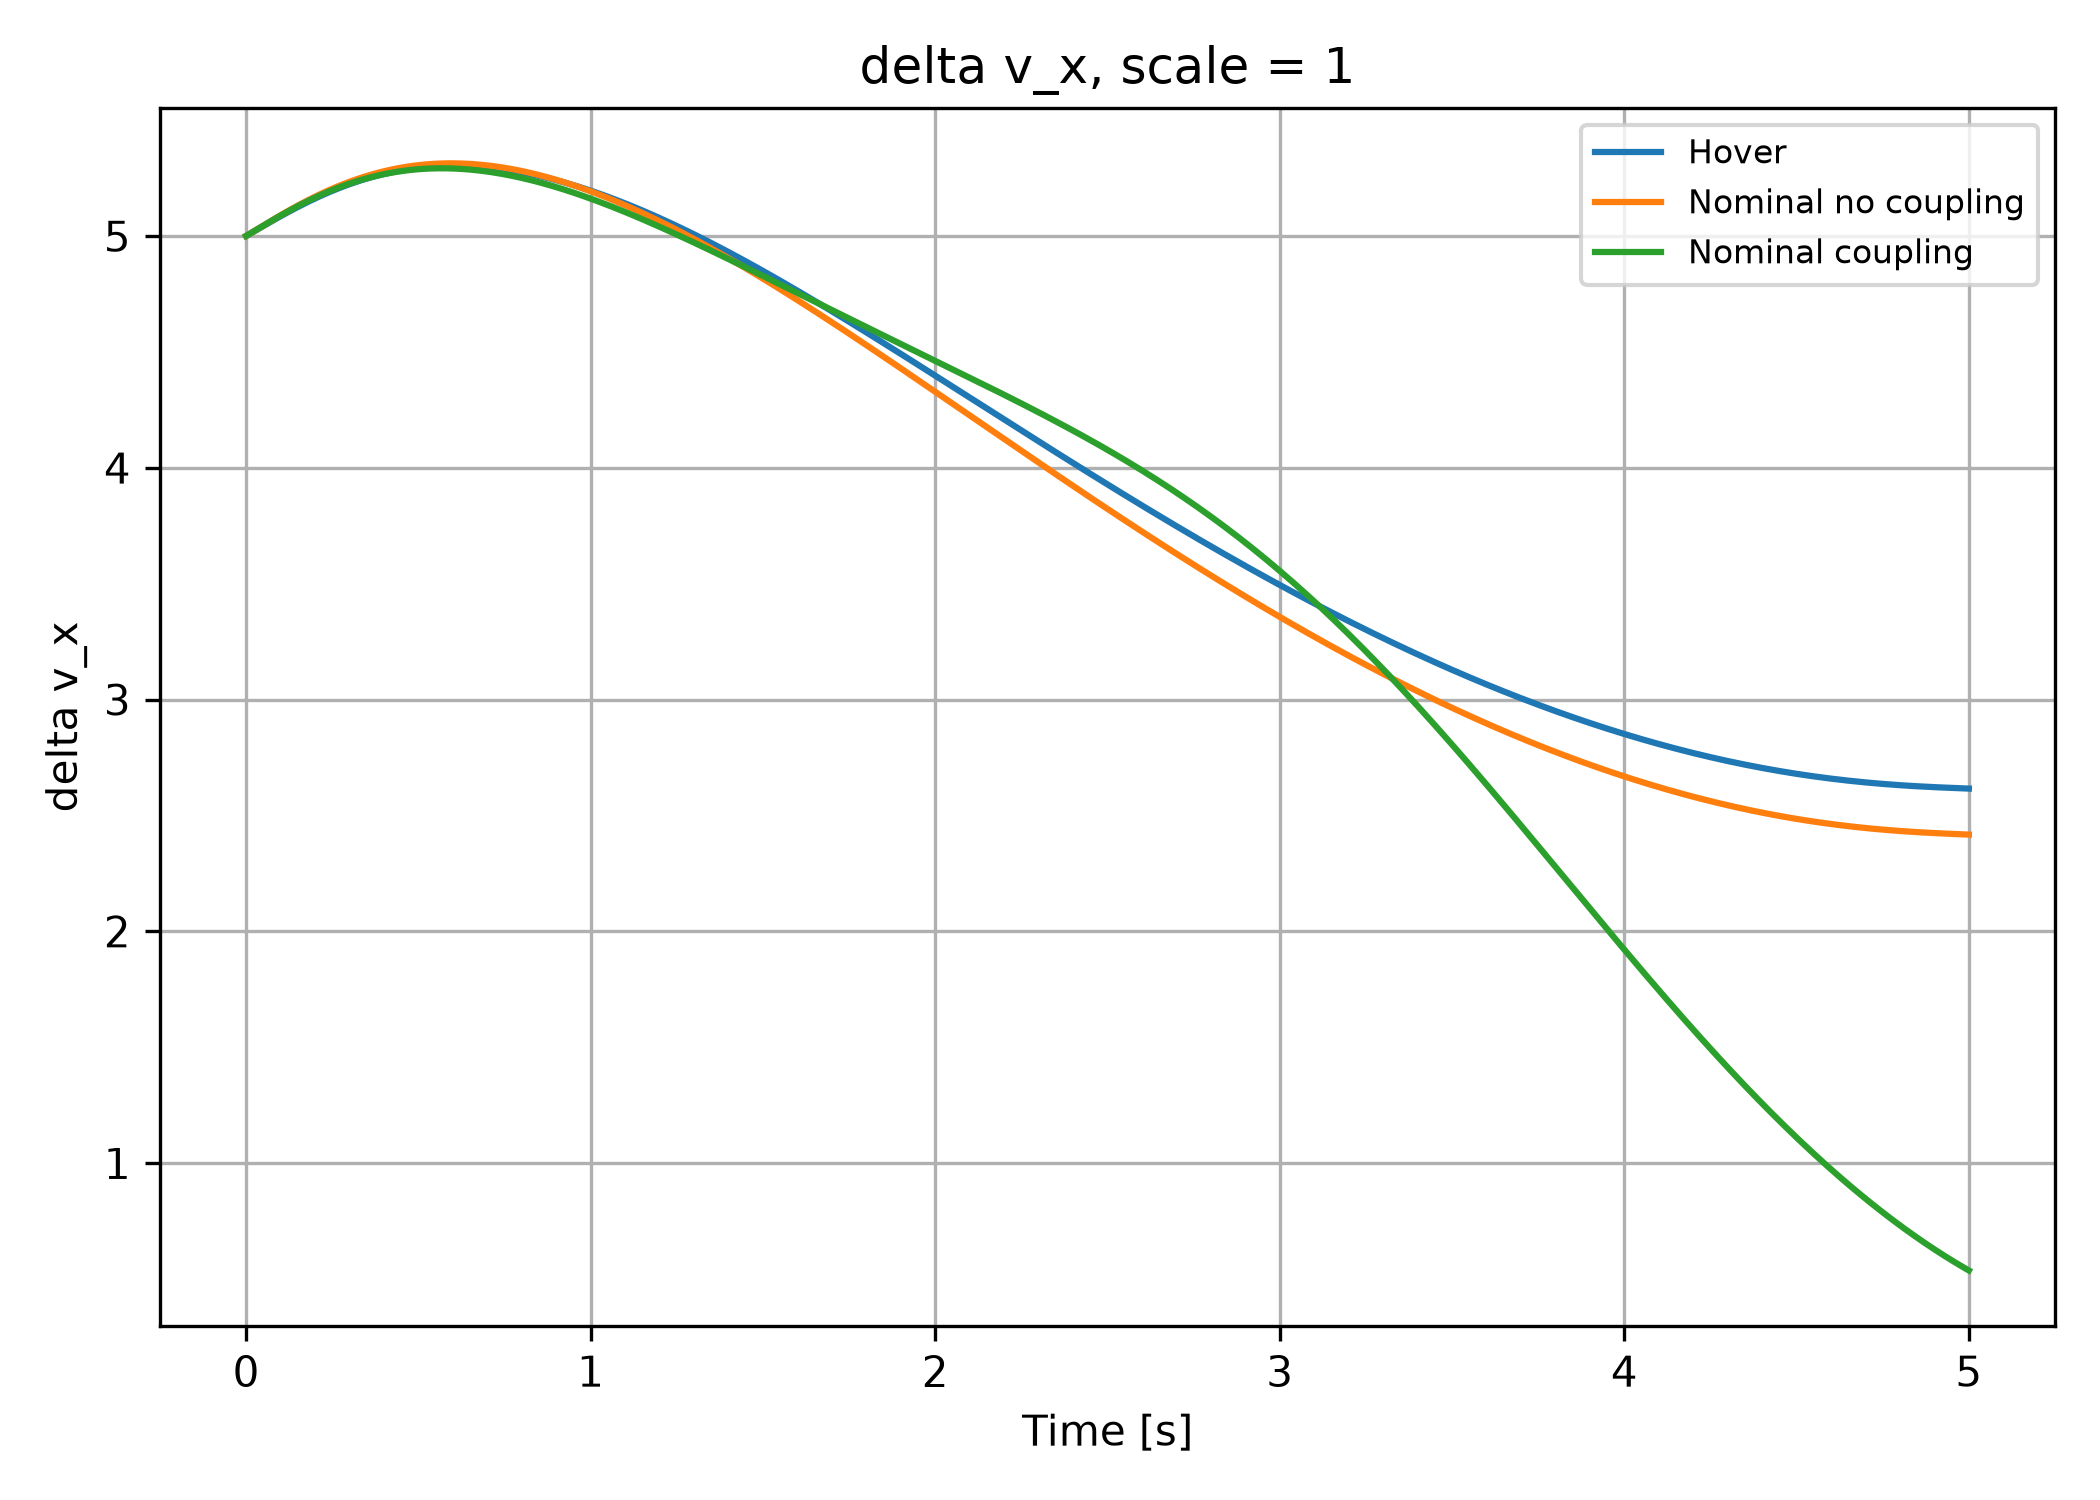
\includegraphics[width=0.90\columnwidth]{sections/PART5C/delta_v_x_time_history_scale_1p0.png}
    \caption{Horizontal velocity perturbation \(\delta v_x(t)\) for perturbation scale \(\gamma=1\).}
    \label{fig:vx-scale1}
\end{figure}
\begin{figure}[htbp]
    \centering
    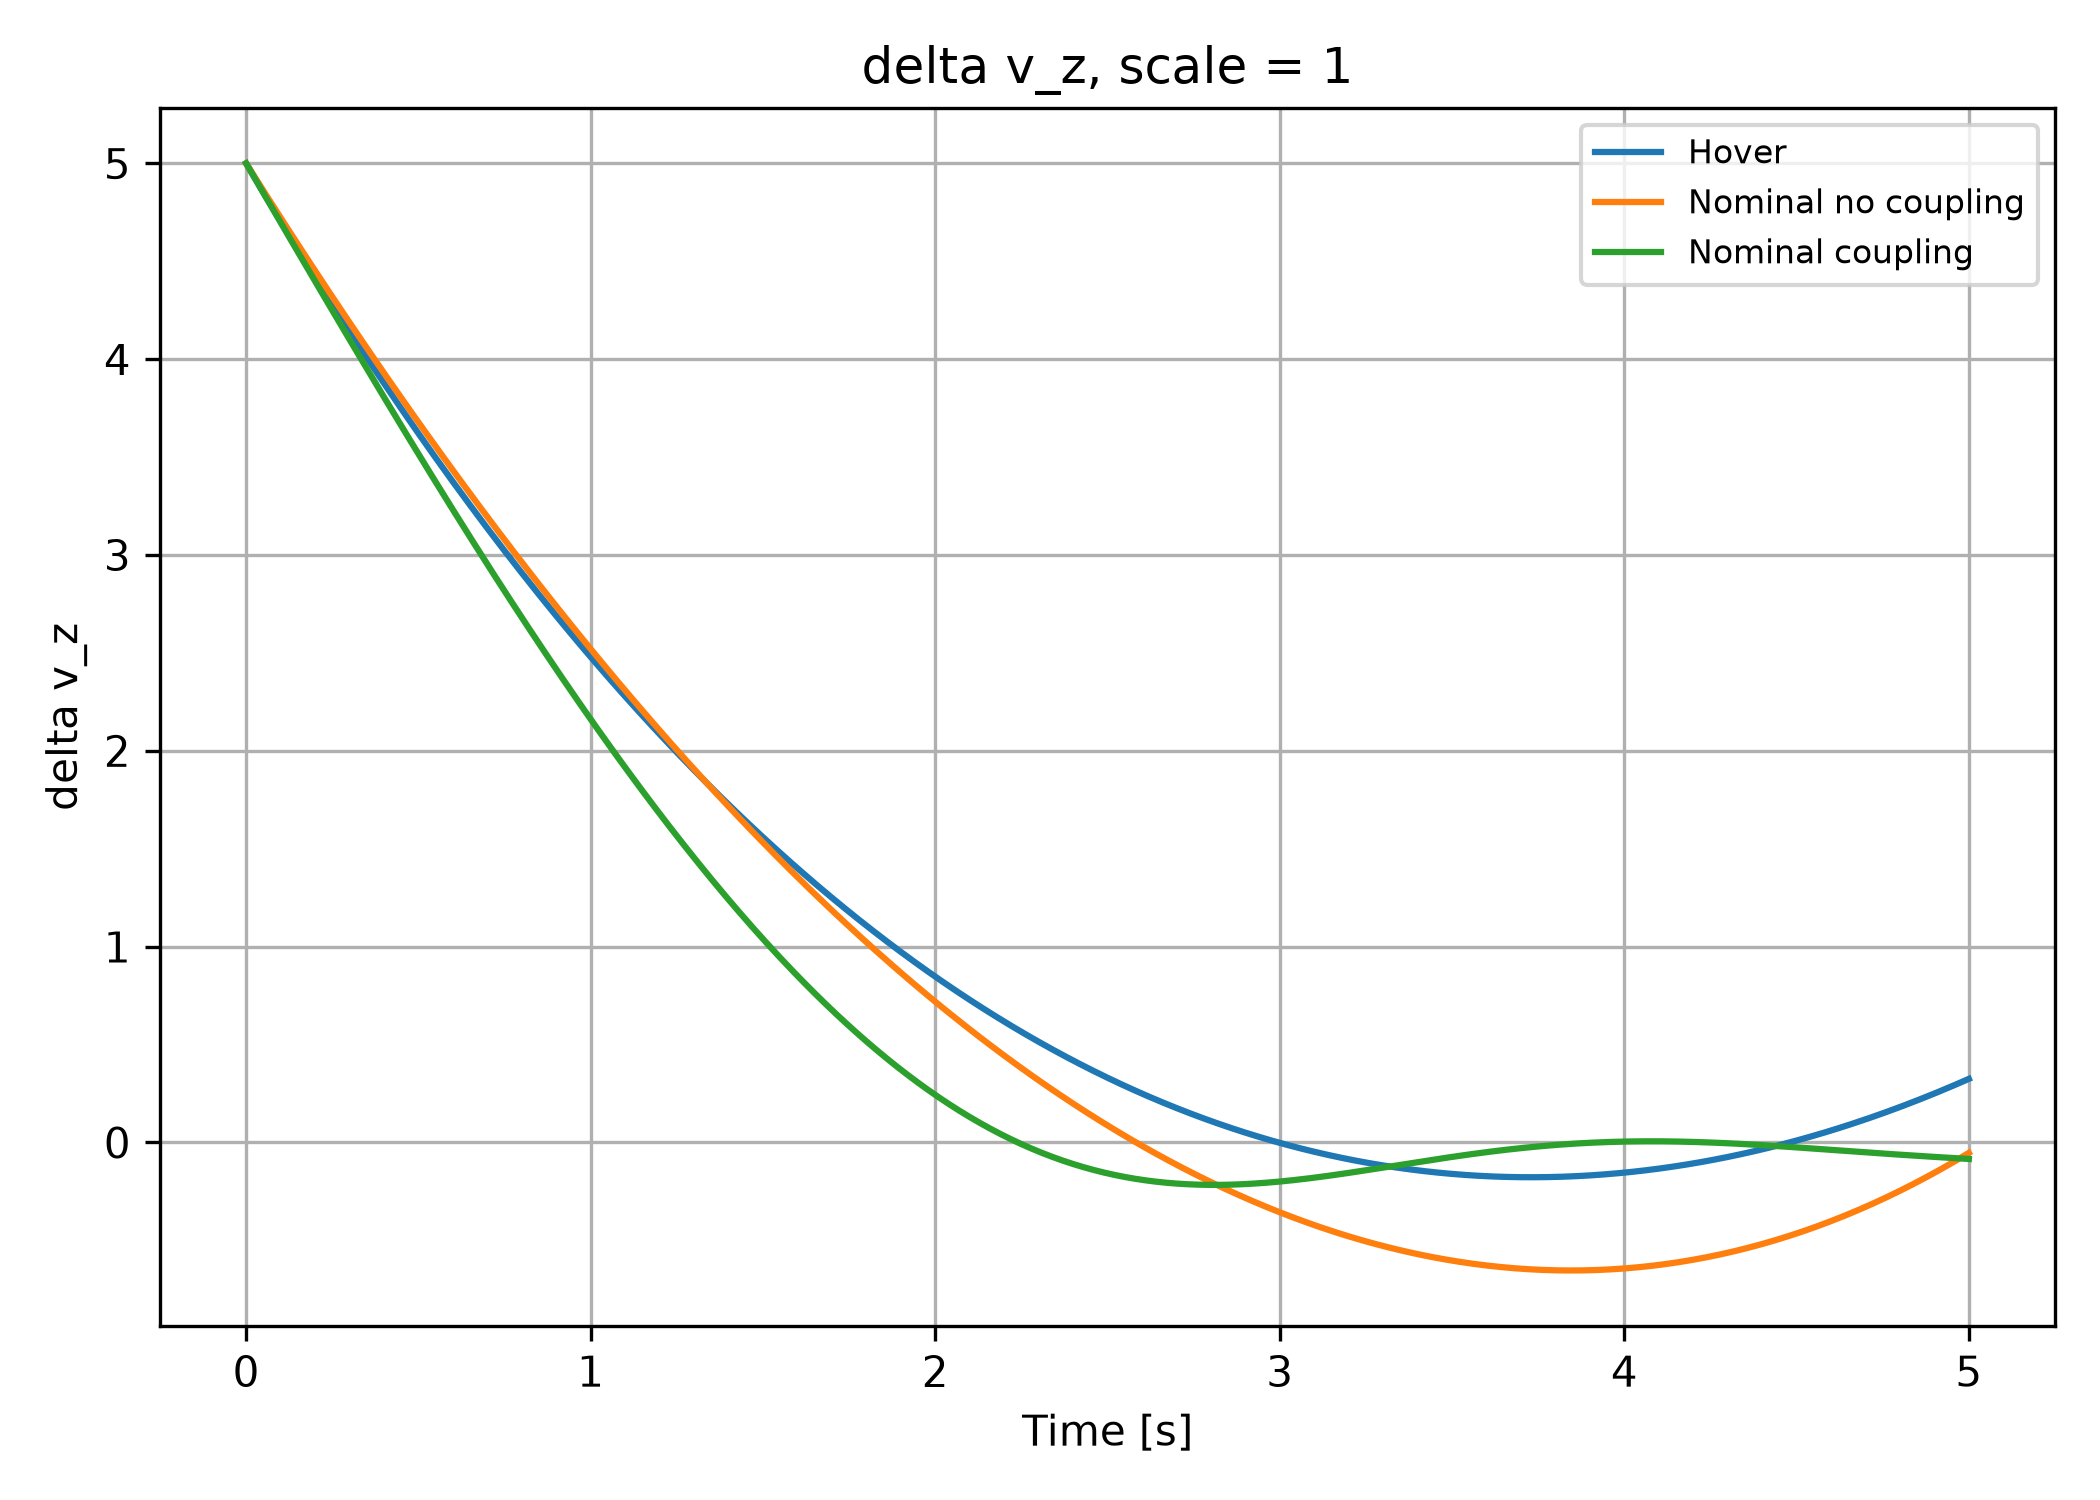
\includegraphics[width=0.90\columnwidth]{sections/PART5C/delta_v_z_time_history_scale_1p0.png}
    \caption{Vertical velocity perturbation \(\delta v_z(t)\) for perturbation scale \(\gamma=1\).}
    \label{fig:vz-scale1}
\end{figure}

\begin{figure}[htbp]
    \centering
    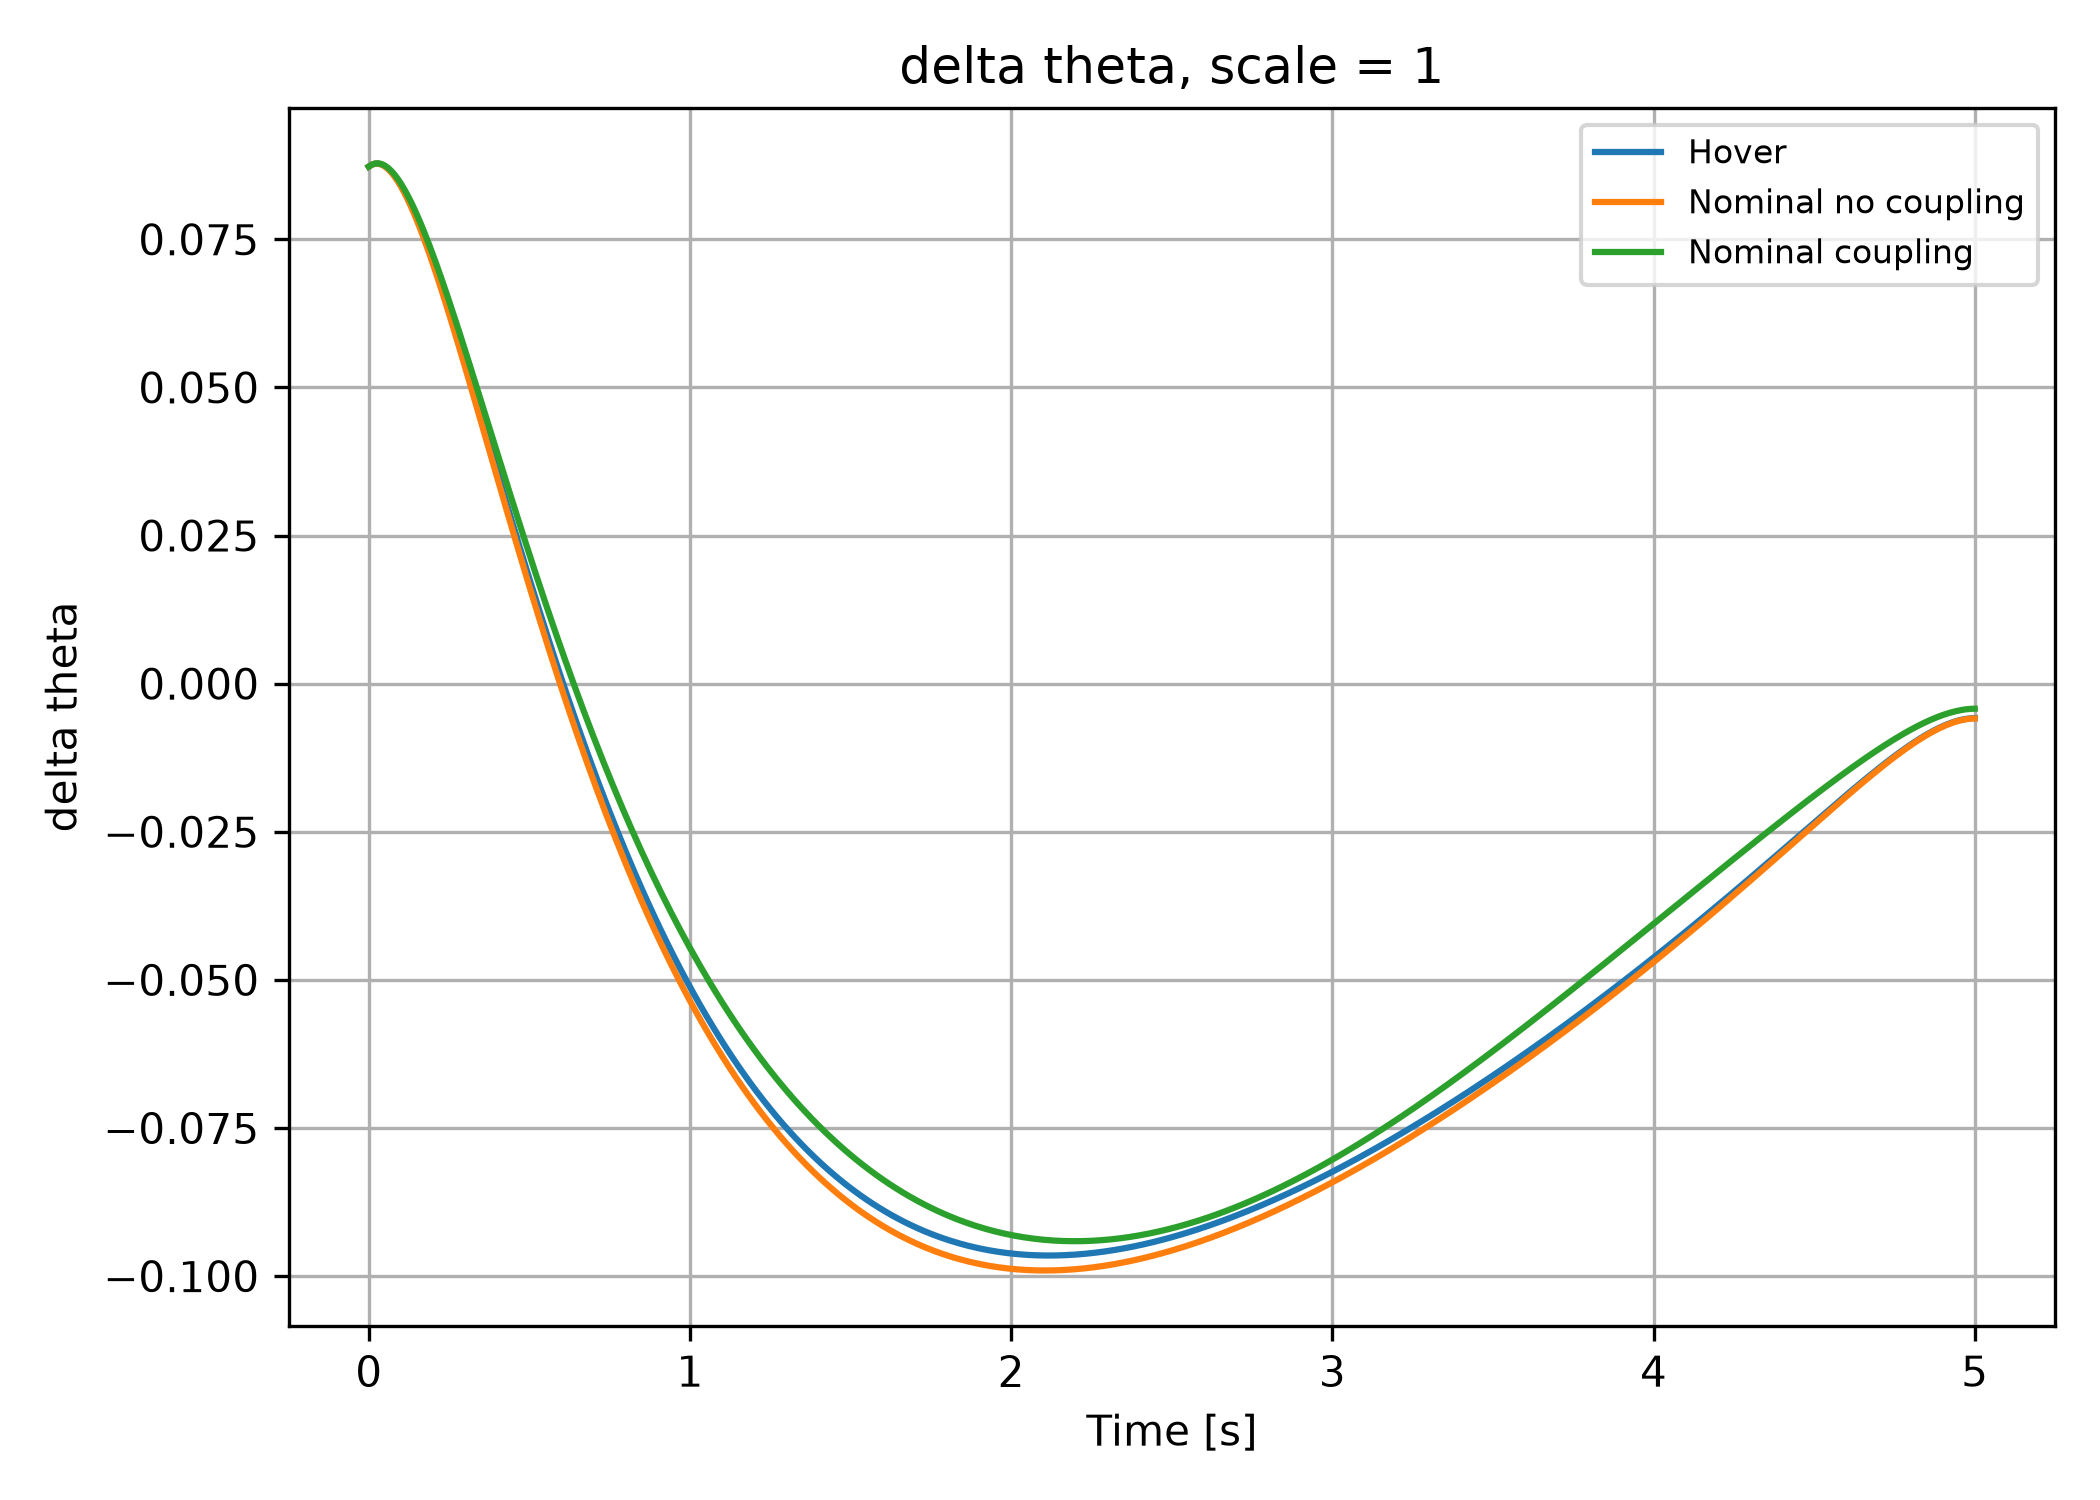
\includegraphics[width=0.90\columnwidth]{sections/PART5C/delta_theta_time_history_scale_1p0.png}
    \caption{Attitude perturbation \(\delta\theta(t)\) for perturbation scale \(\gamma=1\).}
    \label{fig:theta-scale1}
\end{figure}

\begin{figure}[htbp]
    \centering
    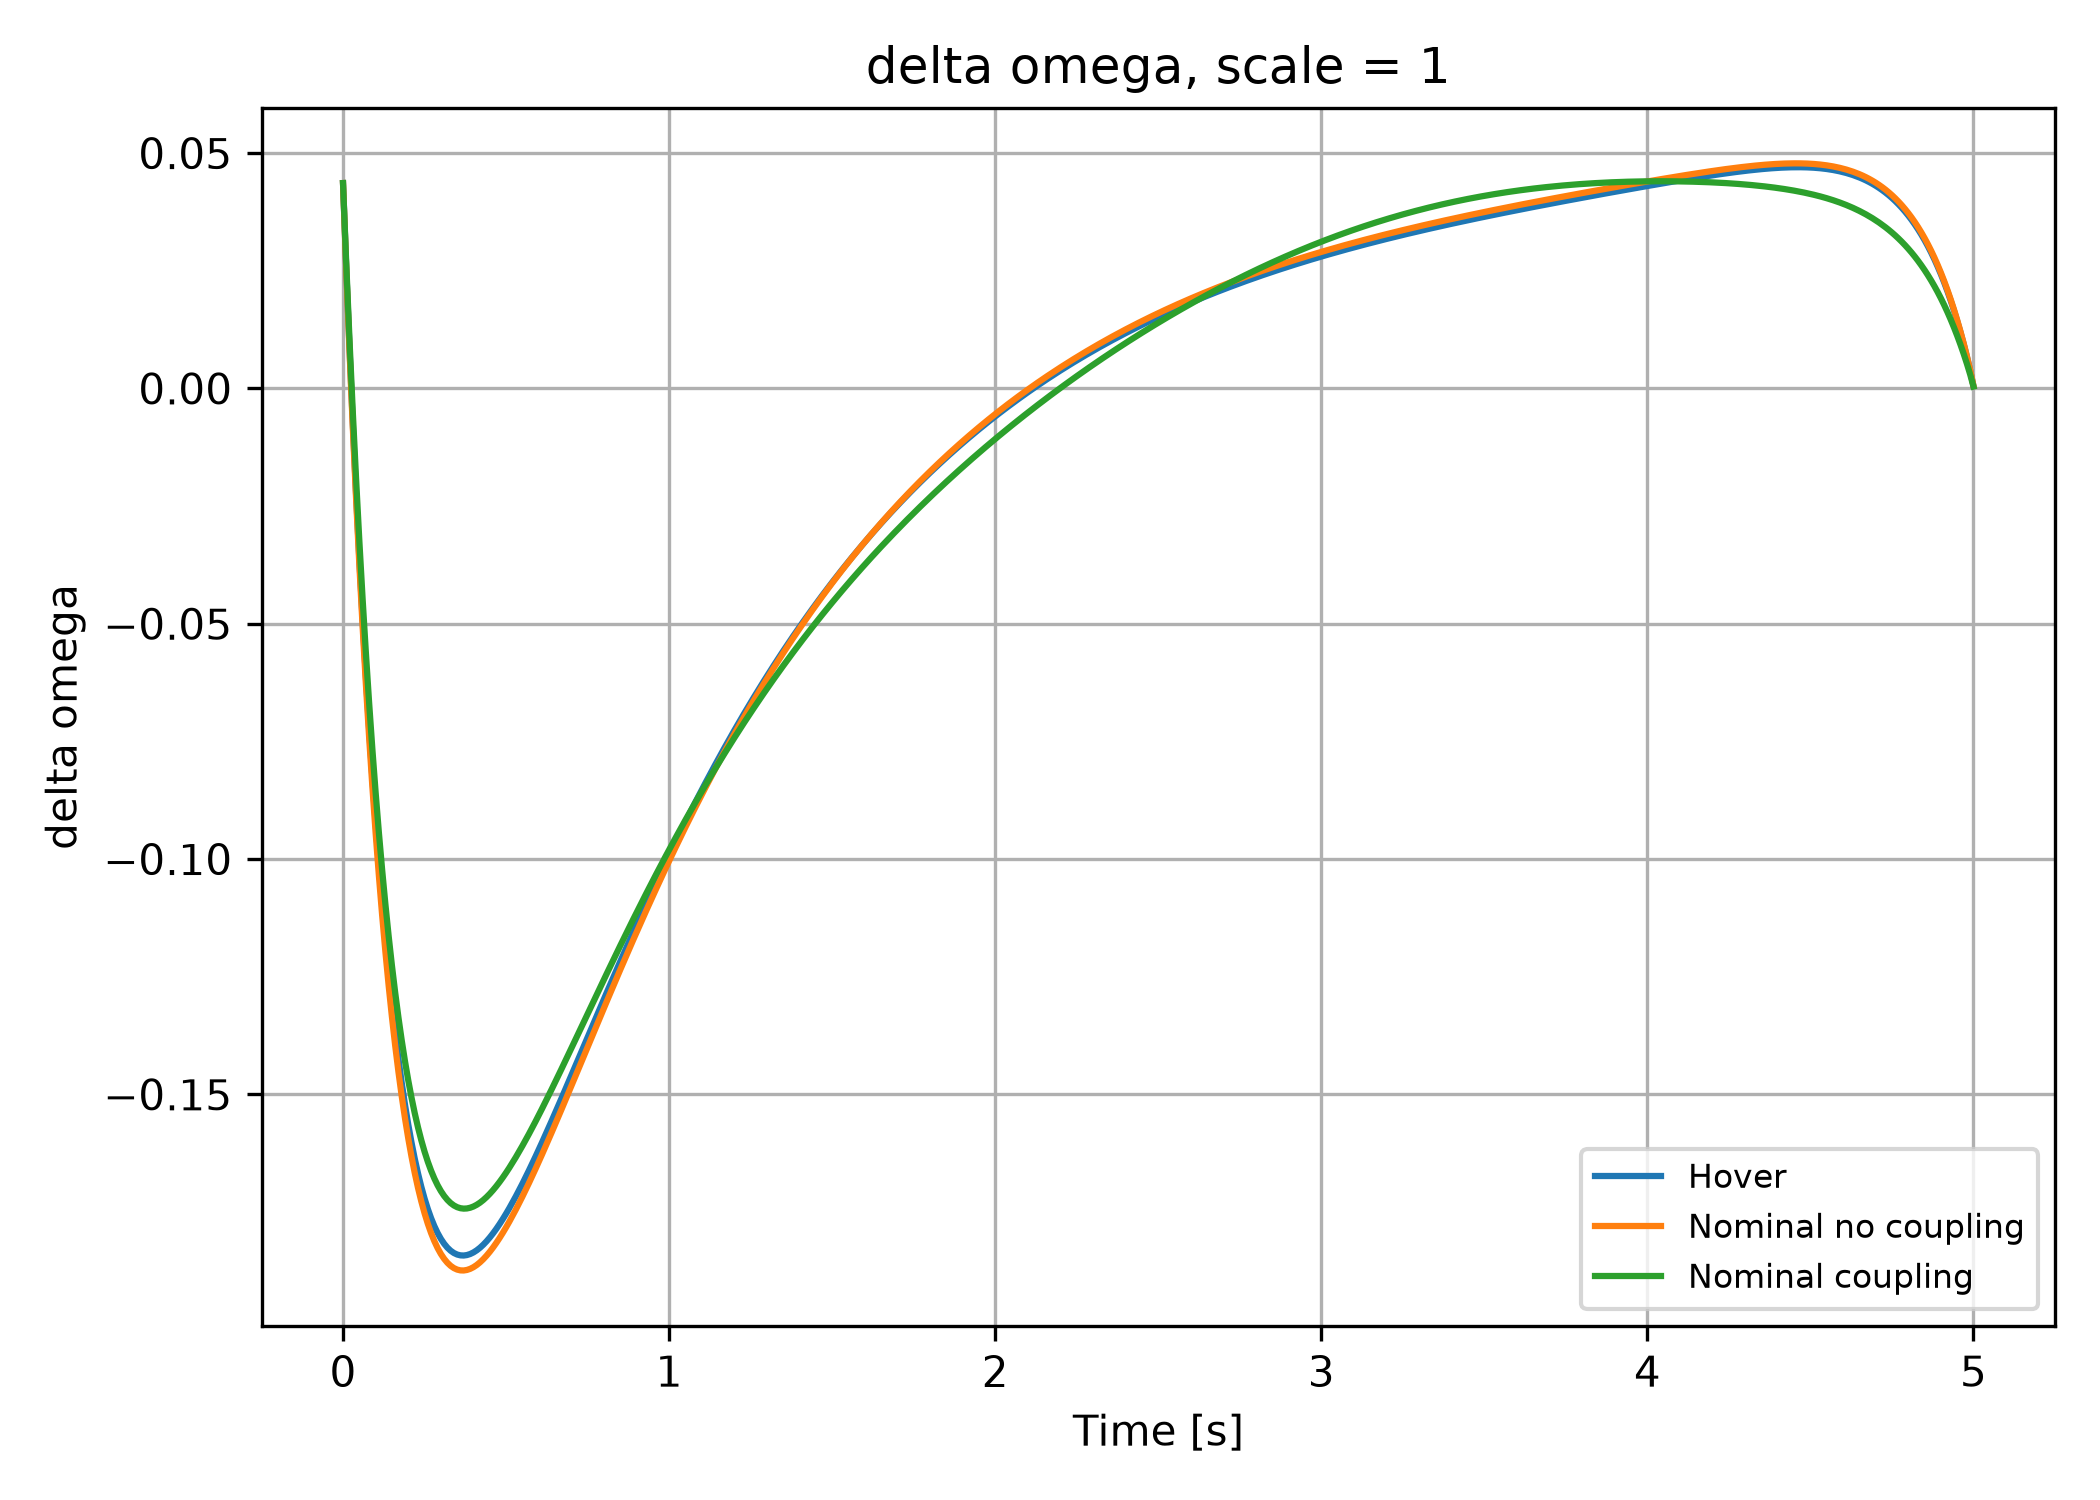
\includegraphics[width=0.90\columnwidth]{sections/PART5C/delta_omega_time_history_scale_1p0.png}
    \caption{Angular velocity perturbation \(\delta\omega(t)\) for perturbation scale \(\gamma=1\).}
    \label{fig:omega-scale1}
\end{figure}

